\documentclass[12pt,a4paper]{report}

\usepackage[spanish]{babel}
\usepackage[utf8]{inputenc}

%%%%%%%%%%%%%%%%%%%%%%%%%%%%%%%%%%%%%%%%%%%%%%%%%%%%%%%%%%%%%%%%%%%%%%%%
%% Fonts 
% \usepackage{fourier}
% \usepackage[scaled=0.83]{helvet} %% Helvetica queda demasiado grande
% \renewcommand{\ttdefault}{txtt}
% \usepackage[scaled=0.9]{inconsolata}
% \usepackage[scaled=0.75]{beramono}
\usepackage{courier}

% \usepackage{graphics} % Or
\usepackage{graphicx} %% and then \includegraphics[scale=0.5,...]{filename}

\setlength{\parskip}{\baselineskip}

\usepackage[spanish]{babel}

\usepackage{hyperref}

\usepackage{listings}

\lstdefinestyle{spec}{
  % lineskip=-0.25ex,
  % belowskip=0.25\medskipamount,
  basicstyle=\sffamily,
  keywordstyle=\bfseries,
  columns=flexible,
}
\lstdefinestyle{code}{
  % lineskip=-0.25ex,
  % belowskip=0.25\medskipamount,
  basicstyle=\ttfamily\small,
  keywordstyle=\bfseries,
}
\newcommand{\lstsetocl}{
  \lstset{
    language=OCL,
    style=spec,
  }
}
\newcommand{\lstsetc}{
  \lstset{
    language=C++,
    style=code,
    literate=,
  }
}
\newcommand{\lstsetpt}{
  \lstset{
    language=progtalk,
    style=spec,
  }
}

\usepackage{todonotes}
\setlength{\marginparwidth}{7em}

\title{Trabajo de Fin de Carrera: Progtalk}
\author{Adrián Bartol Molina}
\date{Febrero de 2011}

\begin{document}
\maketitle
\tableofcontents

\chapter{Introducción}

\todo{AH: intenta tener líneas reales más cortas.}
Este proyecto consiste en el diseño e implementación de una herramienta la cual a partir de una comunicación entre varias entidades (programas, procesos, etc), nos devuelve una representación gráfica de dicha comunicación. \textit{Progtalk} se integra dentro del proyecto \textit{Transformers}, en el cual se estudian varios lenguajes con el objetivo de representar la información de los requisitos del sistema de ferrocarril europeo (ERTMS). En concreto, uno de los lenguajes que se estudia es el de diagramas de secuencia (MSC, \emph{Message Sequence Charts}), y aquí es donde encaja \textit{Progtalk}. \todo{AB:Aquí deberíamos explicar en detalle que papel juega Progtalk en Transformers.}

La labor de nuestra herramienta consiste en, dada una comunicación entre dos o mas entidades, el procesado de esta comunicación y la creación de una representación gráfica de ésta. Para ello podemos describir el funcionamiento de la herramienta en tres fases:

\begin{itemize}
\item Validación léxica y sintáctica del fichero de entrada, el cuál contiene la comunicación,
\item validación semántica, almacenaje de la información parseada, y comprobación de la integridad de la información almacenada, y
\item exportación de la comunicación a un fichero externo de tipo \textit{latex}.
\end{itemize}

\todo{AB:deberíamos hacer que Introducción fuera le capítulo 0 y comenzar numerando a partir del capítulo MSC}
El presente trabajo esta estructurado del siguiente modo. En primer lugar, en el capítulo \ref{ch:msc} se presentan los \textit{Diagramas de Secuencia}, su historia y un resumen de su funcionamiento. Tras esta introducción teórica pasaremos al capitulo \ref{ch:lenguaje}, donde explicaremos en detalle en qué consiste el lenguaje que hemos creado para representar las comunicaciones entrantes a \textit{Progtalk}. En el capitulo \ref{ch:diseno} explicaremos el análisis y diseño que se ha realizado antes de comenzar la implementación de la herramienta. Por último, en el capitulo \ref{ch:conclusiones} se presentan las conclusiones extraídas de la realización de este proyecto, y posibles vías futuras de desarrollo.

\chapter{MSC: Diagramas de secuencia}
\label{ch:msc}

Según Bjorner~\cite{bjorner}, los diagramas de secuencia (a partir de ahora MSCs), son una notación gráfica para describir intercambios de mensajes entre entidades. Los MSCs fueron estandarizados por primera vez por la \textit{CCITT} (conocida ahora como la \textit{ITU-T}) en \textit{Recommendation Z.120} en 1992, donde se especificaron sus componentes. Se realizaron revisiones en 1996, donde se especificó la forma en que varios MSCs (llamados \textit{basic} MSC (BMSC) pueden ser combinados para formar un documento MSC en cual la relación entre dichos BMSCs se describe mediante un \textit{high-level} MSC (HMSC), y en 1999 donde se ofrecen facilidades adicionales para la especificación de los datos que se pasan dentro de los mensajes, y se permiten expresiones en línea.

A continuación vamos a hacer un breve resumen sobre los BMSC, que son los diagramas que vamos a usar en \textit{Progtalk}.

\section{Basic MSCs (BMSCs)}
Un \textit{basic} MSC (a partir de ahora BMSC), esta formado por un conjunto de instancias. Una instancia es una entidad abstracta en la cual suceden eventos. Una instancia se nota con un cuadrado vacío, el cual tiene una linea recta que sale verticalmente y hacia abajo desde su base. Esta recta representa una linea temporal donde los eventos van ocurriendo por orden cronológico de arriba hacia abajo. Los eventos que pueden suceder entre instancias son:

\begin{itemize}
\item Acciones: eventos locales a una instancia. Se representan por una caja en la línea temporal con una etiqueta en su interior. Las acciones se usan para especificar cambios en el estado interno de la instancia,
\item Mensajes salientes: representan el envío de un mensaje a una instancia.
\item Mensajes entrantes: representan la recepción de un mensaje. Lógicamente a cada evento de mensaje saliente le corresponde otro evento de mensaje entrante. A esto se le conoce como intercambio de mensajes y se representa con una flecha que sale de la línea de tiempo de la instancia origen a la línea de tiempo de la instancia destino. Todo intercambio de mensajes debe de estar etiquetado con un identificador. 
\item Condiciones: describen un estado el cual es común a un conjunto de instancias dentro del MSC. Su fin es meramente informativo y se representan mediante hexágonos los cuales se extienden a lo largo de las líneas de tiempo de las instancias sobre las que la condición se aplica. El texto de la condición debe ir en el interior del hexágono.
\item Temporizadores: son locales a las instancias y como su propio nombre indica sirven para controlar la ocurrencia temporal de los eventos. Se nota con un reloj de arena.
\item Procesos de creación de instancias, donde una instancia crea a otra nueva.
\item Procesos de terminación de instancias, donde una instancia se termina a si misma.
\item Corregiones: partes de la línea temporal de una instancia donde la premisa de que los eventos ocurran de forma estrictamente temporal deja de ser indispensable. Se notan con una línea discontinua.
\end{itemize}

En nuestro proyecto solo vamos a usar eventos de mensajes entrantes y salientes. A continuación mostramos un ejemplo como debería representarse gráficamente una comunicación.

%%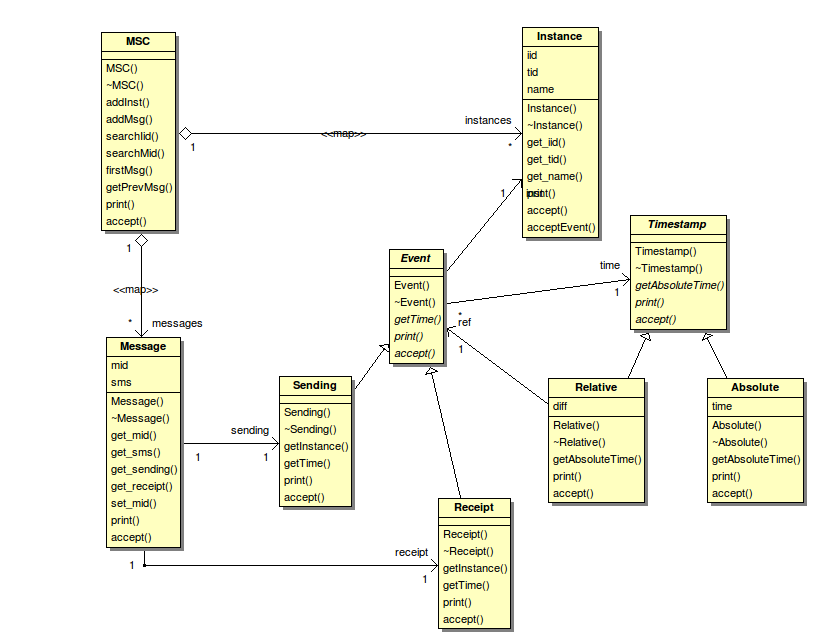
\includegraphics[scale=0.5]{./imagenes/fig1}

Para que nuestros BMSCs sean correctos deben cumplir una serie de requisitos:
\begin{itemize}
\item Los nombres de las instancias deben de ser únicos.
\item Todos los eventos de entrada y salida deben de estar relacionados con una instancia ya declarada en el momento del evento.
\item Los identificadores de los mensajes deben de ser únicos.
\item Un tiempo de envío no pueden ser nunca mayor que su correspondiente tiempo de recepción (ya que no podemos mandar un mensaje hacia atrás en el tiempo).
\todo{ver si es obligatorio que los mensajes sean estrictamente secuenciales o no. AH: no es obligatorio, sólo es necesario comprobar que los mensajes no viajan atrás en el tiempo.}
\end{itemize}

\chapter{Lenguaje}
\label{ch:lenguaje}
\lstsetpt

La herramienta \textit{Progtalk} debe recibir la comunicación en un fichero escrito en un determinado lenguaje que permita representar MSCs. Dicho lenguaje consta de dos secciones:
\begin{itemize}
\item Declaración de instancias, y
\item declaración de mensajes.
\end{itemize}

Cada una de estas declaraciones se llama sentencia, y entre sentencias debe aparecer un símbolo '';''.

Es responsabilidad del usuario traducir la comunicación que quiere pasar a \textit{Progtalk} a este formato.

\section{Instancias}

Las instancias de nuestro lenguaje se describen mediante tres parámetros:

\begin{itemize}
\item Identificador de instancia. Este parámetro debe ser obligatoriamente introducido por el usuario. Ademas debe ser un identificador válido (aquí se entiende como identificador valido un conjunto de caracteres y números que comienza obligatoriamente por una letra).
\item Tipo de la instancia. Este parámetro es opcional, y esta pensado darle una funcionalidad real en un futuro desarrollo.
\item Parámetro \textit{name}. Este parámetro es opcional, y esta pensado darle una funcionalidad real en un futuro desarrollo.
\end{itemize}

El formato del lenguaje es:

\begin{itemize}
\item \lstinline[mathescape]!instance $inst$ of $tinst$ { $pname$ }!
\end{itemize}
donde:
\begin{itemize}
\item \lstinline{instance}, \lstinline{of}, ``\lstinline!{!'' y ``\lstinline!}!'' son palabras reservadas del lenguaje, y
\item $inst$ (identificador de instancia), $tinst$ (tipo de la instancia), y $pname$ (nombre del parámetro) deben ser introducidos por el usuario.
\end{itemize}

Algunos ejemplos de declaración de instancias son:

\begin{lstlisting}
instance a { "A" };
instance b of type { "B" };
instance c of control;
instance d;
\end{lstlisting}

El usuario puede almacenar tantas instancias como desee, pero estas deben tener un identificador de instancia único.

\section{Mensajes}

Los mensajes de nuestro lenguaje se describen mediante seis parámetros:

\begin{itemize}
\item Identificador de mensaje: este parámetro es opcional. En caso de ser introducido debe ser un identificador válido (aquí se entiende como identificador válido cualquier conjunto de letras, números y ''\_'' que comience por una letra,
\item Mensaje: este parámetro es opcional, y almacena el mensaje de texto propiamente dicho. Puede ser cualquier conjunto de caracteres salvo las comillas y que empiece y termine por comillas,
\item Instancia origen del mensaje: este parámetro debe ser obligatoriamente introducido por el usuario, y representa la instancia que envió el mensaje. La instancia a la que se haga referencia en este parámetro, debe de haber sido declarada previamente en esa misma comunicación,
\item Instancia destino del mensaje: este parámetro debe ser obligatoriamente introducido por el usuario, y representa la instancia que recibió el mensaje. La instancia a la que se haga referencia en este parámetro, debe de haber sido declarada previamente en esa misma comunicación,
\item Tiempo de envío: este parámetro es opcional. Representa el momento exacto en que el mensaje fue enviado, y
\item Tiempo de recepción: este parámetro es opcional. Representa el momento exacto en que el mensaje fue enviado.
\end{itemize}

El formato del lenguaje es:

\begin{itemize}
\item \textit{message} (Identificador del mensaje) \{ (Mensaje) \} \textit{from} (Instancia origen del mensaje) \textit{@} (Tiempo de envío) \textit{to} (Instancia destino del mensaje) \textit{@} (Tiempo de recepción)
\end{itemize}

donde,
\begin{itemize}
\item \textit{message}, \textit{from}, \textit{to} y \textit{@} son palabras reservadas del lenguaje, y
\item (Identificador de mensaje), (Mensaje), (Instancia origen del mensaje), (Tiempo de envío), (Instancia destino del mensaje), y (Tiempo de recepción) deben ser introducidos por el usuario.
\end{itemize}

La instancia origen del mensaje y el instante de envío forman un evento de envío, mientras que la instancia destino del mensaje y el instante de recepción forman un evento de recepción.

Es importante que nos detengamos un momento a explicar en detalle los parámetros de los mensajes relativos a los tiempos de envío y recepción. Estos tiempos pueden ser absolutos o relativos.

\subsection{Tiempos Absolutos}

Entenderemos como tiempos absolutos los siguiente casos:

\begin{itemize}
\item Si el usuario da específicamente un valor absoluto, o
\item si estamos hablando del instante de envío del primer mensaje de la comunicación y el usuario no ha introducido dicho parámetro. En este caso consideraremos siempre un valor absoluto de cero. 
\end{itemize}

Un ejemplo del uso de tiempos absolutos es:

\begin{verbatim}
message m1 { "hola" } from programaA @ 2 to programaB @ 5;
\end{verbatim}

donde el mensaje \textit{m1} consiste en el envío del mensaje \textit{''hola''} de la instancia \textit{programaA} en el instante \textit{2} y la recepción del mensaje en la instancia \textit{programaB} en el instante \textit{5}.

\subsection{Tiempos relativos}

Por otro lado entenderemos por tiempos relativos los siguiente casos:

\begin{itemize}
\item Relativo implícito: si el usuario no da específicamente un valor en cuyo caso calcularemos el parámetro como el instante del ultimo evento (ya sea envío del mensaje actual, o recepción del mensaje anterior) mas una unidad. Por ejemplo:
\begin{verbatim}
message m1 { "hola" } from programaA @ 2 to programaB;
\end{verbatim}
Aquí el tiempo de recepción del mensaje se calcula a partir del mensaje de envío más una unidad, es decir, que el instante de recepción en \textit{programaB} es \textit{3}.
\item Relativo explicito simple: si el usuario aporta un valor del tipo (\textit{+unidad}) donde \textit{unidad} es un numero entero, pero no especifica un evento de referencia. En este caso calcularemos el parámetro como el instante del ultimo evento (ya sea envío del mensaje actual, o recepción del mensaje anterior) mas el valor introducido por el usuario (\textit{+unidad}). Por ejemplo:
\begin{verbatim}
message m1 { "hola" } from programaA @ 2 to programaB @ +3;
\end{verbatim}
Aquí el tiempo de recepción del mensaje se calcula a partir del mensaje de envío más \textit{3}, es decir, que el instante de recepción en \textit{programaB} es \textit{5}.
\item Relativo explicito complejo: si el usuario aporta un evento de referencia y un valor del tipo (\textit{+unidad}) donde \textit{unidad} es un numero entero. El evento de referencia especificado por el usuario puede referirse a un evento de envío o de recepción, y debe de pertenecer a un mensaje ya almacenado anteriormente en esa comunicación. En este caso calcularemos el parámetro como el instante en que ocurrió el evento que especifico el usuario sumándole el valor (\textit{+unidad}) especificado también por el usuario. Cabe destacar que existe la posibilidad de que sólo se introduzca el evento de referencia y que no se introduzca un valor del tipo (\textit{+unidad}), en cuyo caso consideraremos dicho valor (\textit{+unidad}) como +0. Por ejemplo:
\begin{verbatim}
message m1 { "hola" } from programaA @ 2 to programaB @ +5;
message m2 { "adiós" } from programaB @ m1!+3 to programaA @ m1?;
\end{verbatim}
Aquí el tiempo de envío se calcula sumándole al tiempo de envío del mensaje \textit{m1} (es decir, \textit{2}) el valor \textit{+3} dando como resultado \textit{5}. El tiempo de recepción se calculará sumándole al tiempo de recepción de \textit{m1} (es decir, \textit{7})), el valor \textit{+0} dando como resultado \textit{7}.
\end{itemize}

Como último detalle decir que entre sentencia y sentencia (

\section{Sintaxis Concreta}

La gramática, en formato EBNF (\emph{Extended Backus-Naur Form}) es la siguiente:
\begin{verbatim}
//------------------------------------------------------------
//
//  GRAMÁTICA
//    
//    msc ::= inst_decl* message*
//    inst_decl ::= INSTANCE iid |
//                  INSTANCE iid OF tid; |
//                  INSTANCE iid {string}; |
//                  INSTANCE iid OF tid {string};               
//    message ::= MESSAGE mid_opt string_opt origin destiny;
//    mid_opt ::= LAMBDA | mid
//    string_opt ::= LAMBDA | {string}
//    origin ::= LAMBDA | origin_opt
//    origin_opt ::= FROM iid time_ref_opt
//    destiny ::= LAMBDA | destiny_opt
//    destiny_opt ::= TO iid time_ref_opt
//    time_ref_opt ::= LAMBDA | @ time_ref
//    time_ref ::= abs_time | rel_time
//    abs_time ::= num
//    rel_time ::= ref dif_time_opt | dif_time
//    ref ::= mid ! | mid ?
//    dif_time_opt ::= LAMBDA | dif_time
//    dif_time ::= + num | - num
//    iid ::= ID
//    tid ::= ID
//    mid ::= ID
//    string ::= STRING
//    num ::= NUM
//
//------------------------------------------------------------
\end{verbatim}

\chapter{Diseño}
\label{ch:diseno}

\section{Sintaxis Abstracta}
\lstsetocl

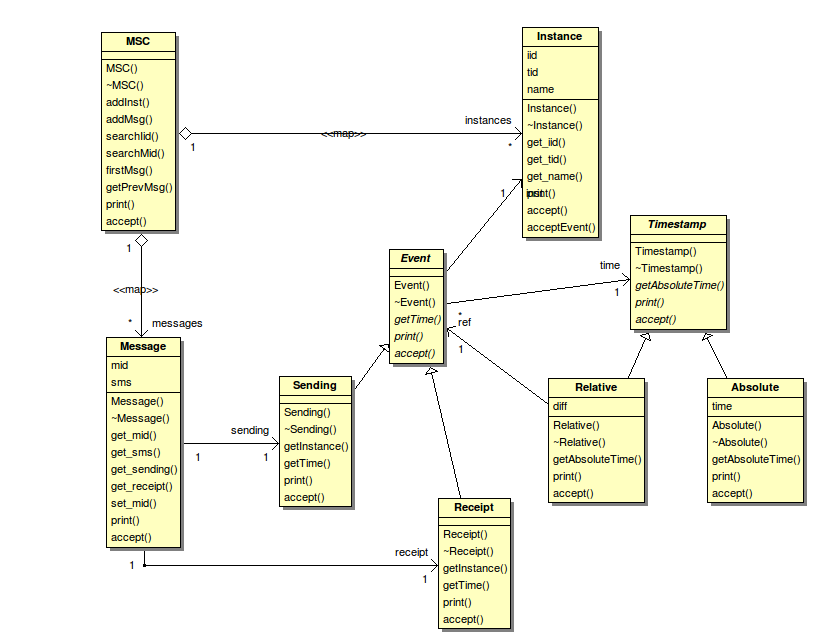
\includegraphics[scale=0.5]{./images/fig2}

La clase \lstinline{Event} es una clase abstracta de la que heredan bla bla bla En C++ vamos a generar la clase \lstinline[style=code,language=C++]{Event} \todo{AH: es sólo un ejemplo de uso de lstinline}.

\verb~"Hola\"$"~ \todo{AH: ejemplo para generar los strings sin necesidad de escapar los comandos latex.}.


\section{Arquitectura}

Básicamente la arquitectura de \textit{Progtalk} es la siguiente:
\begin{itemize}
\item En un primer lugar tenemos el analizador léxico. Su labor es ir tomando información del fichero de entrada carácter a carácter e ir agrupando en \textit{tokens} (unidad mínima de información que maneja posteriormente el analizador sintáctico).
\item Los tokens son enviados al analizador sintáctico, el cuál se encarga de parsear el fichero de entrada (es decir, va uniendo los tokens que va recibiendo y verifica que el fichero entrante esta escrito conforme al lenguaje diseñado para describir el universo del problema).
Durante el análisis sintáctico del fichero de entrada se hace necesario la creación de una serie de objetos los cuales sirven como almacenamiento intermedio de la información. La razón para hacer esto es la siguiente: imaginemos que estamos parseando una línea del fichero de entrada. Lo que el analizador sintáctico (a partir de ahora \textit{parser})va a hacer es ir comparando la entrada con cada una de las reglas de dicho parser. Se irá creando un árbol sintáctico conforme avanza el parseo, y almacenando la información leída para que una vez se acepte la línea de entrada tengamos toda la información sobre dicha línea recopilada, y podamos almacenarla en el objeto\textit{msc} en el cual se almacena toda la comunicación antes de generar el fichero \textit{.tex}.
%% 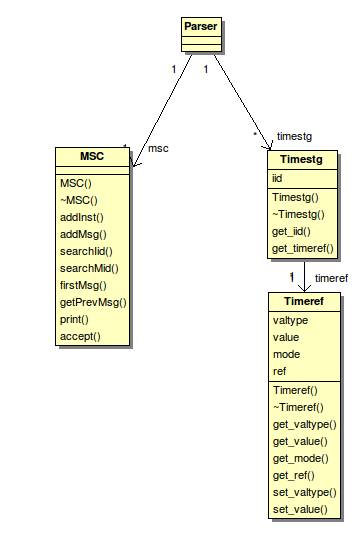
\includegraphics[scale=0.5]{./images/fig3.tiff}

\item Para verificar la consistencia de la comunicación tenemos el analizador semántico. En este punto, debemos explicar que parte de este análisis se ha realizado durante el análisis sintáctico, y parte se ha realizado tras la finalización de éste. La razón por la que tomamos esta decisión es que algunas verificaciones de consistencia, como por ejemplo la no duplicidad de identificadores, era fácil de empotrar dentro del código del analizador sintáctico, optimizando el funcionamiento de \textit{Progtalk} sin aumentar la complejidad del código, mientras que otras verificaciones como por ejemplo la consistencia de los tiempos de envío y recepción, eran suficientemente complejas como para diferir su procesado, simplificando así mucho el código.
\item Por ultimo tenemos el generador de código, que lee toda la comunicación procesada y almacenada en memoria, y la exporta al formato requerido por el usuario.
\end{itemize}

\section{Análisis Léxico}
Para implementar el analizador léxico (al cual hemos llamado \textit{Scanner}) hemos usado flex++. Los tokens que hemos definido para el universo de nuestro problema son:

\begin{itemize}
\item NUM: cualquier número entero.
\item ID: cualquier identificador comenzado en letra y formado por letras, números o el símbolo ''\_''.
\item WHITE: cualquier espacio en blanco o tabulador.
\item STRING: cualquier conjunto de caracteres entre comillado salvo comillas o salto de línea.
\item EOLN: uno o más saltos de línea.
\item INSTANCE: el literal ''instance".
\item OF: el literal "of".
\item MESSAGE: el literal "message".
\item FROM: el literal ''from''.
\item TO: el literal ''to''.
\item AT: el literal ''@''.
\item PLUS: el literal ''+''.
\item MINUS: el literal ''-''.
\item EXCLAMATION: el literal ''!''.
\item INTERROGATION: el literal ''?''.
\item SEMICOLON: el literal '';''.
\item LEFT\_BRACE: el literal ''\{''.
\item RIGHT\_BRACE: el literal ''\}''.
\end{itemize}

\section{Análisis Sintáctico}

Para implementar el analizador sintáctico (al cual hemos llamado \textit{Parser}) hemos usado \textit{bisonc++}. El proceso de parseo es el siguiente. El objeto \textit{Parser} va tomando los tokens enviados por \textit{Scanner} y comprueba que el lenguaje que esta leyendo es un lenguaje correcto. En caso de no serlo se aborta el proceso de parseo y el programa termina.

Las acciones semánticas en \emph{bisonc++} simplemente construyen los
nodos del árbol de sintaxis abstracta. Veamos un ejemplo de una de nuestras acciones semánticas:
\lstsetc
\begin{lstlisting}
message:
     MESSAGE mid_opt string_opt origin_opt destiny_opt SEMICOLON EOLN
        { 
	      string * mid = $2;
          string * desc = $3;
          Timestg * orig = $4;
          Timestg * dest = $5;
        }
	  if (mid == NULL)
	    mid = new string("No_Info_Available");

	  if (desc == NULL)
	    desc = new string("");

	  if (orig == NULL)
	    {
	      std::cout << "ERROR: User didn't provide message's origin" 
			<< std::endl;
	      exit(-1);
	    }

	  if (dest == NULL)
	    {
	      std::cout << "ERROR: User didn't provide message's destiny" 

			<< std::endl;
	      exit(-1);
	    }
	     addMsg(*mid, *desc, orig->get_iid(), dest->get_iid(), 
		 orig->get_timeref(), dest->get_timeref());
	}
;
\end{lstlisting}

Se puede observar cómo el símbolo no terminal \lstinline{message} bla bla bla

\section{Análisis Semántico}

En nuestro programa parte del análisis semántico se realiza de forma paralela al análisis sintáctico y parte se realiza tras finalizar éste. En concreto, las inconsistencias que se reconocen durante el análisis sintáctico son:
\begin{itemize}
\item La declaración de varias instancias con igual identificador,
\item la declaración de varios mensajes con igual identificador,
\item la ausencia de elementos imprescindibles de un mensaje, como su origen o destino,
\item la referencia a un mensaje o instancia que no ha sido declarado anteriormente.
\end{itemize}

El hecho de detectar estas inconsistencias nada más producirse, nos da la ventaja de evitar el procesado de una comunicación errónea, ahorrando tiempo y recursos.

Una vez terminado este proceso con éxito, pasamos a la segunda parte del análisis semántico donde comprobaremos la consistencia en los tiempos de envío y recepción de los mensajes. Hay dos razones por las que nos hemos realizado esta comprobación en paralelo con el análisis sintáctico:
\begin{itemize}
\item Por un lado, durante la fase de análisis del problema, tomamos la decisión de intentar almacenar la información del fichero de entrada tan fielmente como fuera posible para así poder dar marcha atrás si lo deseáramos y obtener de nuevo el fichero de entrada a partir del la información parseada y almacenada. Esto implica que los tiempos relativos se almacenan como referencias y no como valores absolutos, lo que hace imposible comprobar su integridad hasta el final del parseo,
\item y por otro lado, comprendimos que el código del analizador sintáctico se volvería demasiado complejo y poco legible si finalmente incluíamos este tipo de verificaciones durante esta fase.
\end{itemize}

Para la implementación de esta parte del analizador semántico hemos usado un patrón \textit{Visitor}~\cite{gof}.

\section{Generación de Código}

Para esta tarea hemos utilizado un patrón de diseño \textit{Visitor}, el cual recorre toda la información almacenada y a partir de ésta crea un fichero \textit{.tex} que compilado en \textit{latex} nos dará una representación gráfica de la comunicación.

\chapter{Conclusiones y Trabajo Futuro}
\label{ch:conclusiones}

\bibliography{biblio.bib}
\bibliographystyle{plain}

\end{document}
